\section{Definizione del problema}
Nel capitolo precedente è stato illustrato un metodo atto all'identificazione delle frecce che rientrano nel campo visivo della camera. Viene ora trattato come sia possibile ottenere la posizione della freccia, precedentemente ottenuta, nelle coordinate 3D (U,V,W) rispetto alla base del robot.

\begin{figure}[H]
	\centering
	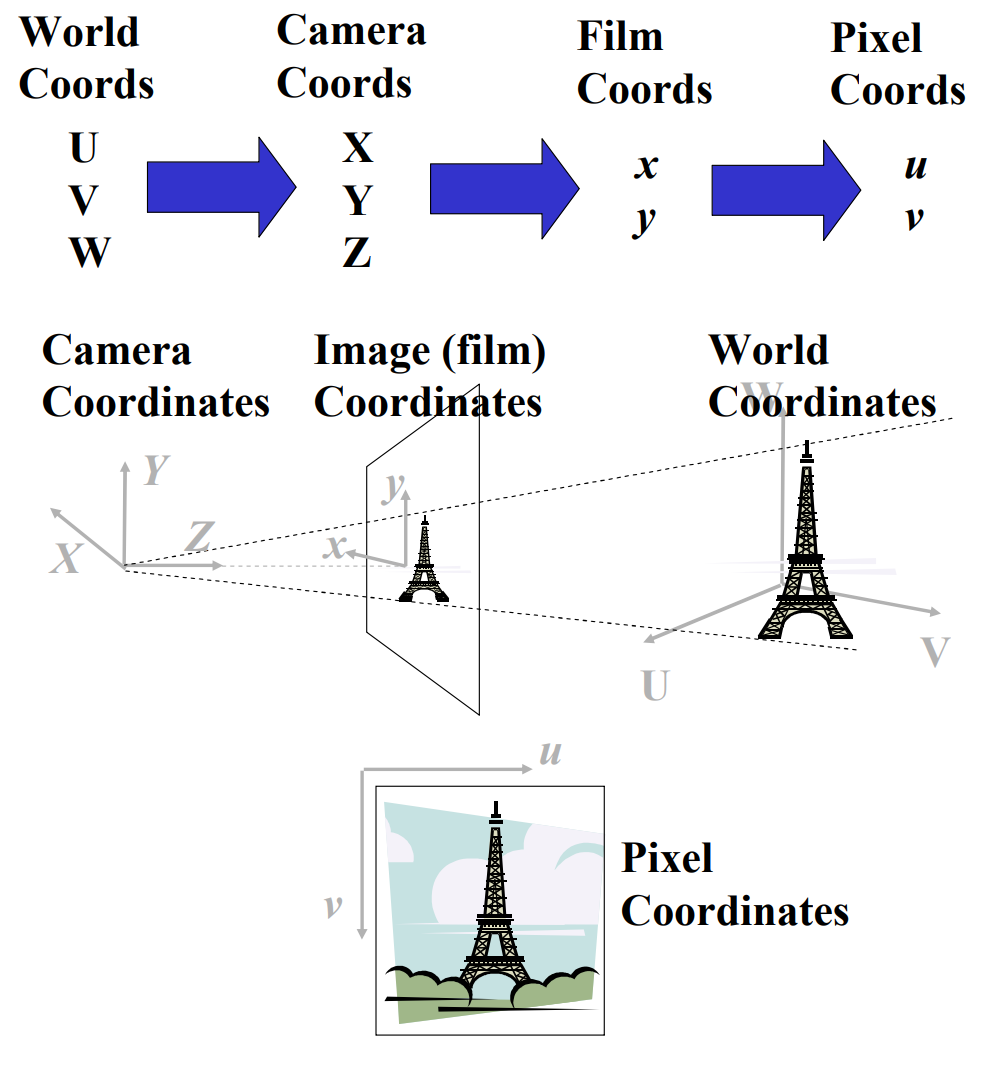
\includegraphics[width=0.8\textwidth]{Immagini/world_coords.png}
	\caption{Schema concettuale delle diverse coordinate}
	\label{fig:fromcamtoworld}
\end{figure}

Come si vede in Fig.\ref{fig:fromcamtoworld} si devono effettuare tre trasformazioni per ottenere a partire dalle world coordinates le pixel coordinates.
Il problema, nel caso specifico preso in considerazione dal report, risulta essere l'opposto: dalle coordinate nella camera è necessario ottenere la posizione globale dell'oggetto effettuando una trasformazione inversa.
Si analizzeranno ora le singole trasformazioni che permetteranno alla fine di ottenere il risultato voluto.

\section{Da wolrd coordinates to camera coordinates}
\begin{figure}[H]
	\centering
	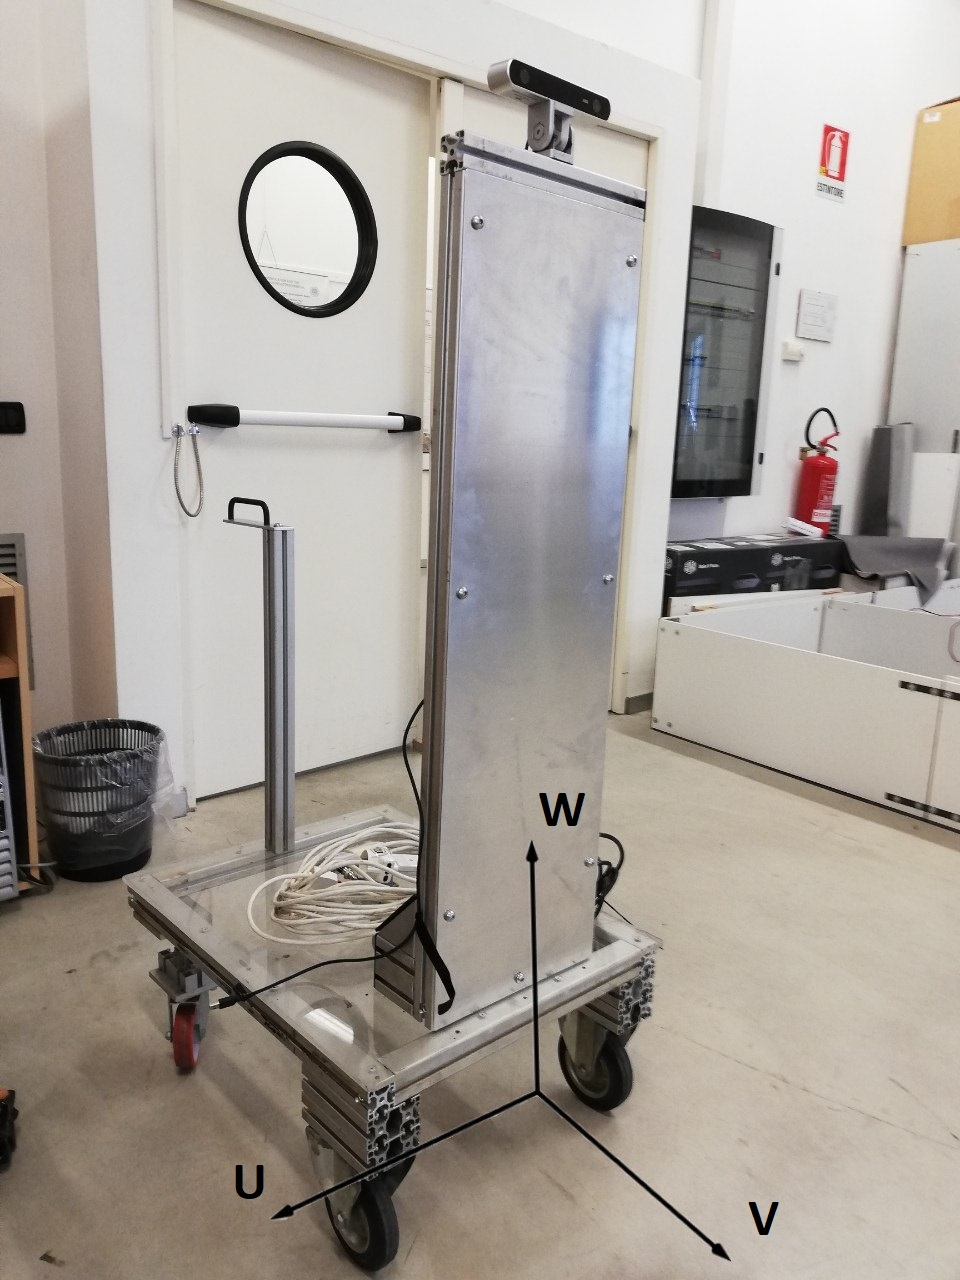
\includegraphics[width=0.4\textwidth]{Immagini/SupportoCamera_asse1.jpg}
	\caption{Posizione del world frame}
	\label{fig:worldframe}
\end{figure}

Partendo da un sistema di riferimento solidale al robot e all'altezza del pavimento, che identifichiamo come sistema globale, è possibile definire una matrice di rototraslazione per ottenere il sistema di riferimento solidale al centro della camera.
\begin{equation*}
R_{worldcam} = R_{traslazione}*R_{rotazione} =\\
\begin{pmatrix}
1 & 0 & 0 & 0 \\
0 & 1 & 0 & 0 \\
0 & 0 & 1 & h_{cam} \\
0 & 0 & 0 & 1 \\
\end{pmatrix}*
\begin{pmatrix}
cos(\dfrac{\pi}{2}+\alpha) & -sin(\dfrac{\pi}{2}+\alpha) & 0 & 0 \\
sin(\dfrac{\pi}{2}+\alpha) & cos(\dfrac{\pi}{2}+\alpha)& 0 & 0 \\
0 & 0 & 1 & 0 \\
0 & 0 & 0 & 1 \\
\end{pmatrix}
\end{equation*}

È stata effettuata una traslazione lungo l'asse W in quanto la camera è posta esattamente sopra all'origine del sistema $O_{UVW}$ ed una rotazione rispetto all'asse U di $ \dfrac{\pi}{2}$ in quanto, per convenzione, si associa all'asse delle Z la profondità nel frame solidale alla camera.
A questo punto è necessario effettuare un'altra rotazione di $\alpha$ gradi rispetto all'asse X a seconda dell'inclinazione alla quale si sceglie di far lavorare la camera
INSERISCI LA FOTO DELLA CAMERA SUL PALO PER FAR CAPIRE IL CONCETTO!!!!!!!!!!!!!!!!!!!!!!!!!!!

\section{Da camera coordinates a film coordinates}
\begin{figure}[H]
	\centering
	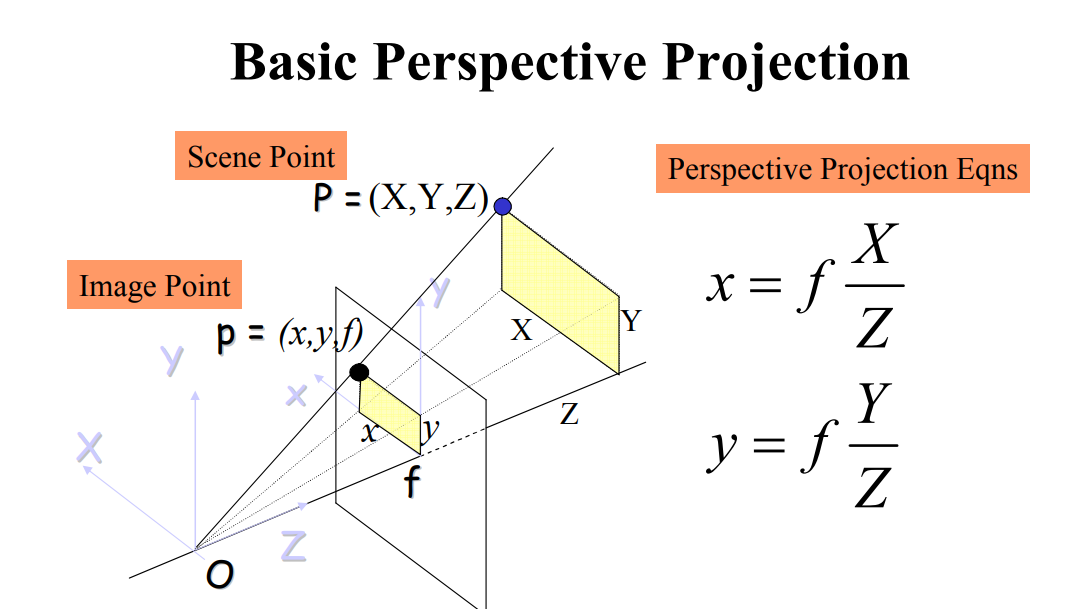
\includegraphics[width=0.7\textwidth]{Immagini/perspective_projection.png}
	\caption{Descrizione del problema}
	\label{fig:perspective_projection}
\end{figure}
In Fig.\ref{fig:perspective_projection} \textit{f} rappresenta il fuoco della camera, parametro ottenibile attraverso una procedura di calibrazione.

\section{Da film coordinates a pixel coordinates}

\begin{figure}[H]
	\centering
	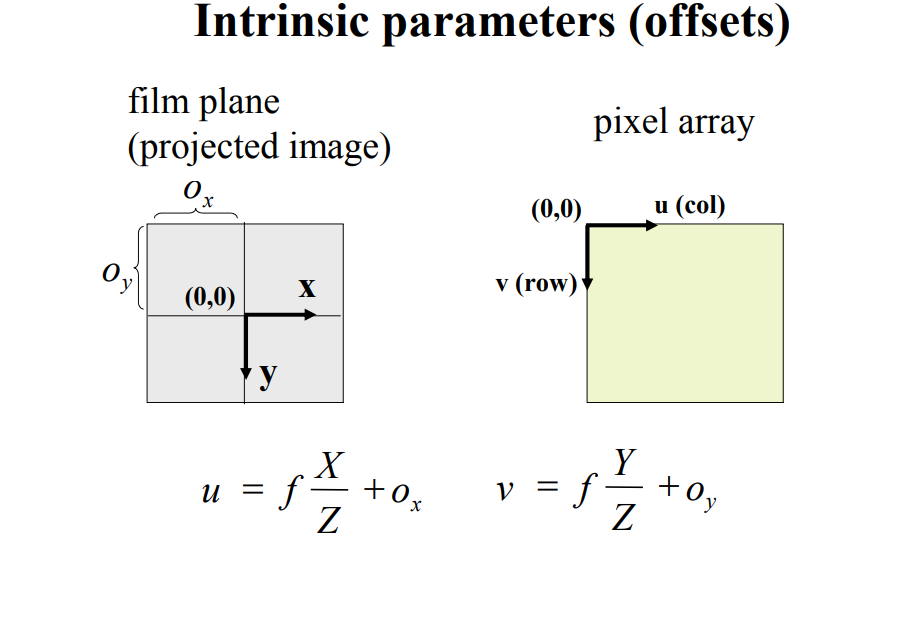
\includegraphics[width=0.7\textwidth]{Immagini/intrinsic_parameters.png}
	\caption{Descrizione dell'ultima trasformazione}
	\label{fig:intrinsic_parameters}
\end{figure}
In Fig.\ref{fig:intrinsic_parameters} $ O_{x}$ e $ O_{y} $ sono anch'esse ricavabili tramite la procedura di calibrazione della camera

\section{Problema al rovescio}
\begin{figure}[H]
	\centering
	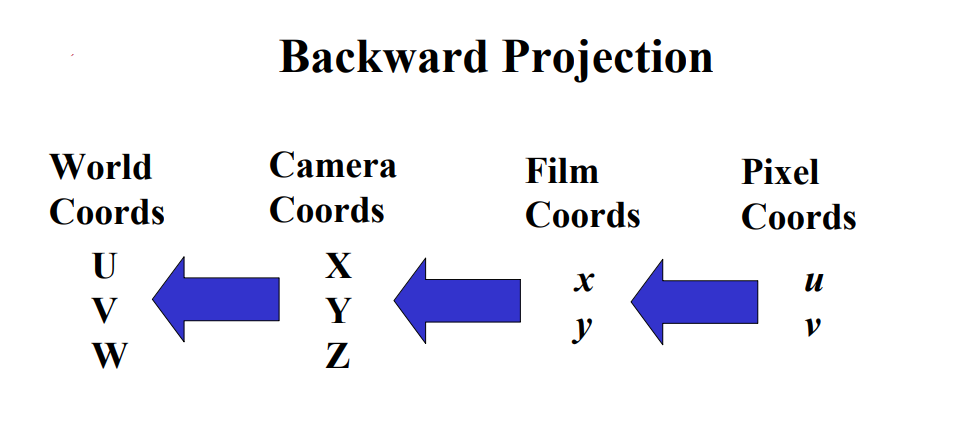
\includegraphics[width=0.7\textwidth]{Immagini/backward.png}
	\caption{Problema inverso}
	\label{fig:backward}
\end{figure}

Come si vede in Fig.\ref{fig:backward} si deve ora affrontare il processo inverso siccome, nel caso trattato, si hanno a disposizione \textit{u} e \textit{v} e si vogliono ottenere \textit{U,V,W}.
Come già detto prima $ O_{x}$ e $ O_{y} $ e \textit{f} sono ottenibili tramite calibrazione;dunque:
\begin{equation}
\begin{split}
x = u -O_{x}\\
y = v -O_{y}
\end{split}
\end{equation}

Sono state ottenute le equazione del film coordinates. È ora necessario ottenere le camera coordinates. Per fare ciò è necessario conoscere il valore di Z, cosa ottenibile in due modi:
\begin{itemize}
	\item \textbf{} utilizzando una camera con sensore di profondità
	\item \textbf{} assumendo che gli oggetti siano sempre posti su un piano di cui si conosce l'equazione.
\end{itemize}
La seconda assunzione è, nella realtà dei fatti, una ipotesi corretta in quanto gli oggetti e le frecce giaceranno sempre sul pavimento.
È quindi richiesto di calcolare l'equazione del pavimento nel camera frame:
\begin{itemize}
	\item \textbf{}
		\begin{equation}
			\begin{split}
			z = 0
			\end{split}
		\end{equation}
		rappresenta l'equazione del piano se fosse nel world frame
	\item \textbf{}
		\begin{equation}
		\begin{split}
		z*R_{worldcam} = 0
		\end{split}
		\end{equation}
		il piano così calcolato è la descrizione dal punto di vista matematico del pavimento dal punto di vista della camera
	\begin{figure}[H]
		\centering
		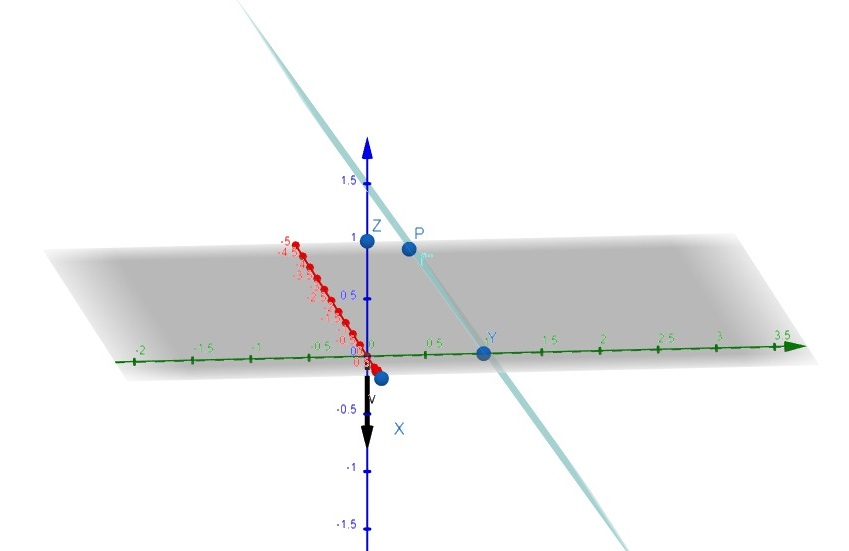
\includegraphics[width=0.7\textwidth]{Immagini/piano_camera.jpeg}
		\caption{Piano del pavimento nel camera frame}
		\label{fig:piano_camera}
	\end{figure}
	\item \textbf{}
	si può dunque calcolare il fattore di scala s dato un generico piano $ax+by+cz+d=0$
		\begin{equation}
		\begin{split}
		\dfrac{-d}{aX'+bY'+c}\\	
		\end{split}
		\end{equation}
	dove
		\begin{equation}
		\begin{split}
		X'=\dfrac{x}{f}=\dfrac{X}{Z}\\
		Y'=\dfrac{y}{f}=\dfrac{Y}{Z} \\
		\end{split}
		\end{equation}
	che sono le coordinate normalizzate rispetto a Z.
	\item \textbf{}
	Dunque, come ultimo passaggio si moltiplica tutto per il fattore di scala:
		\begin{equation}
		\begin{split}
		X=X'*s\\
		Y=Y'*s\\
		Z=S
		\end{split}
		\end{equation}
	
\end{itemize}

Per ottenere le equazione nel world frame si deve dunque utilizzare la matrice inversa:

$$
\begin{pmatrix}
U  \\
V  \\
W  \\
1  \\
\end{pmatrix}
=R_{worldcam}^{-1}*
\begin{pmatrix}
X  \\
Y  \\
Z  \\
1  \\
\end{pmatrix}
$$
